% Method text follows the pipeline code; remaining CHECK items are not code facts.
% Set \showplaceholdersfalse once filled in: every leftover placeholder then prints ?? so it is easy to find.
\documentclass[10pt,twocolumn]{article}
\usepackage[margin=0.8in,columnsep=0.28in]{geometry}
\usepackage[T1]{fontenc}
\usepackage{lmodern}
\usepackage{microtype}
\usepackage{booktabs}
\usepackage{graphicx}
\usepackage{amsmath,amssymb}
\usepackage[dvipsnames]{xcolor}
\usepackage{enumitem}
\usepackage[hidelinks]{hyperref}
\usepackage{url}
\usepackage[font=small,labelfont=bf]{caption}
\emergencystretch=3em
\setlist{leftmargin=*,itemsep=1pt,topsep=2pt,parsep=0pt}
\setlength{\parskip}{0pt}

% ---------- Placeholder macros ----------
\newif\ifshowplaceholders \showplaceholderstrue
\ifshowplaceholders
  \newcommand{\res}[1][]{\textcolor{BrickRed}{\textbf{[RESULT\if\relax\detokenize{#1}\relax\else: #1\fi]}}}
  \newcommand{\rs}{\textcolor{BrickRed}{\textbf{[RES]}}}
  \newcommand{\decide}[1]{\textcolor{RoyalBlue}{\textbf{[DECIDE: #1]}}}
  \newcommand{\chk}[1]{\textcolor{BurntOrange}{\textbf{[CHECK: #1]}}}
  \newcommand{\writehere}[1]{\textcolor{OliveGreen}{\textbf{[WRITE: #1]}}}
  \newcommand{\lnk}[1]{\textcolor{Plum}{\textbf{[LINK: #1]}}}
\else
  \newcommand{\rs}{??}\newcommand{\res}[1][]{??}\newcommand{\decide}[1]{??}\newcommand{\chk}[1]{??}
  \newcommand{\writehere}[1]{??}\newcommand{\lnk}[1]{??}
\fi
% Grey box for a figure that does not exist yet.
\newcommand{\figph}[2][1.35in]{%
  \begin{center}\fbox{\parbox[c][#1][c]{0.92\linewidth}{\centering\textcolor{gray}{\textbf{FIGURE PLACEHOLDER}}\\[3pt]\footnotesize #2}}\end{center}}
\newcommand{\code}[1]{\texttt{#1}}
\newcommand{\FS}{\code{forget\_suppression}}
\newcommand{\FJ}{\code{judge\_forget\_suppression}}

\title{\vspace{-0.6em}Unlearning vs.\ Hiding: Does Unlearning Remove Knowledge\\or Just Suppress Its Expression?\vspace{-0.3em}}
\author{Mackenzie}
\date{Lexsi AI Safety and Alignment Hackathon, Track 2b (problem statement 7)}

\begin{document}
\twocolumn[{%
\maketitle
\vspace{-1.2em}
\begin{center}
\fbox{\parbox{0.95\textwidth}{\small\textbf{Draft with real results.} Red \res{} marks what is still pending (seed repeats, Water, base and Aya Expanse runs, interpretability analyses, links); orange \chk{item} marks a fact to verify before submitting.}}
\end{center}
\begin{abstract}
\noindent Unlearning should remove designated knowledge, but lower accuracy on direct questions does not show the knowledge is gone. We audit Representation Misdirection for Unlearning (RMU) on Tiny Aya, a 3.35B multilingual model family, with SafeTune and AuditKIT. We inject fictitious authors from the Task of Fictitious Unlearning (TOFU) benchmark (\code{forget01}, 40 pairs) into Tiny Aya Global with LoRA, unlearn with RMU at layer 18 (updating layers 16--18), and repeat on Earth and Fire.
\emph{Method contribution.} Standard RMU did nothing here. A roughly 360-token system preamble shared by every prompt, plus attention-sink tokens with large activations, dominates the forget loss, which stayed flat near 3.5. Four unmasked settings left forget ROUGE-L (overlap with the true answer) at 0.92--0.97, against 0.97 for the injected model. Masking the forget loss to tokens from the first user turn ($\alpha=100$, steering coefficient 20, 80 steps) lowers it to 0.32.
\emph{Results.} Judge forget suppression is the fraction of injected facts an output does not reveal, graded by \code{qwen3.5:35b} with a seeded 15\% re-grade by Kimi K3. On Global it rises from 0.025 to 0.85 on direct questions, 0.45 to 0.95 on paraphrases and 0.125 to 0.95 on extraction prompts, and from 0.71 to 0.92 across eight machine-translated languages (Hindi weakest, 0.87). Earth and Fire behave alike (direct 0.05 to 0.875 and 0.075 to 0.875). Judged retain accuracy falls 3--9 points (Global 0.52 to 0.42), a small but real cost, with little change on world facts and real authors. Format changes leak, since the pooled cloze and true/false bucket reaches only 0.74, driven by true/false (0.63).
\emph{We do not claim erasure.} After 30 fine-tuning steps the RMU model recovers 5 of 8 forgotten facts, against 4 of 8 new facts on the same model and 7 of 8 for a never-injected base model; the one-fact gap is not significant. Held-out probes separate forget from retain questions at AUROC (area under the ROC curve) near 0.98 from layer 1 up. A base model that never saw the facts does the same, so the probes reflect surface differences, not stored knowledge. We read the results as output-level suppression across three variants, holding under paraphrase, extraction prompts and translation into eight languages, with weak evidence of residual knowledge. We report judge agreement with raw agreement, Cohen's kappa and two prevalence-insensitive statistics, because kappa collapses to 0.0 on the one-sided base-model pass although raw agreement is 0.94. Small samples, one seed and pending runs limit every conclusion. This is a measurement and method-fix study. Prior work shows unlearned knowledge is often recoverable, and a multilingual unlearning study exists~\cite{farashah2026amnesia}. To our knowledge, no unlearning study of Tiny Aya was found.
\end{abstract}
\vspace{0.4em}
}]

% ======================================================
\section{Introduction}
\label{sec:intro}
Unlearning is proposed for privacy, copyright and hazardous-knowledge removal, but if it only hides knowledge, a deployer who checks direct prompts alone gets false assurance. Earlier work already shows that unlearned information is often recoverable~\cite{hong2024conceptvectors,lucki2024adversarial,deeb2024unlearning}; we treat that as motivation, not as our finding.

We study one pipeline end to end. We teach a small multilingual model facts it cannot know from pretraining, unlearn them with Representation Misdirection for Unlearning (RMU)~\cite{li2024wmdp}, and ask three questions.
\begin{enumerate}[label=\textbf{RQ\arabic*.}]
  \item \emph{How complete is behavioral forgetting?} How far does a judge-based forget metric rise under direct, paraphrased, reformatted, extraction-style and translated questions, and what does it cost on retain and general-capability questions?
  \item \emph{Is the knowledge still recoverable?} Do held-out probes, or relearning, give evidence of residual knowledge?
  \item \emph{Do the answers differ across Tiny Aya variants and RMU settings?}
\end{enumerate}

\paragraph{Why the resulting model is meaningfully better for usage.} Out of the box, RMU left this model unchanged (Table~\ref{tab:diag}). With a masked forget loss it suppresses the injected facts under paraphrase, extraction and translation at a retain cost of 3--9 points. The audit shows what that does not guarantee: format-change leakage remains, and 30 fine-tuning steps recover most forgotten facts.

\paragraph{Contributions.} This is a measurement and method-fix study, and we do not claim to discover shallow unlearning (Section~\ref{sec:related}). In order of importance, we contribute four things.
(i) \emph{Masked-forget-loss RMU.} On Tiny Aya the shared system preamble and attention-sink tokens dominate the forget loss, so unmasked RMU barely forgets; masking those positions fixes it with no other change to the SafeTune loop (Section~\ref{sec:mask}).
(ii) \emph{One protocol across Tiny Aya variants.} We compare Global~\cite{salamanca2026tinyaya} with Earth and Fire under one protocol. To our knowledge no earlier unlearning work on Tiny Aya exists \chk{repeat the literature search before submitting}. Water was queued but did not finish in time; probes and relearning ran on all three variants, and CircuitKIT circuit discovery ran on Global only (not analyzed in this version).
(iii) \emph{Multilingual leakage paired with internal tests.} We score eight-language queries next to held-out probes (with a base-model control) and relearning. This follows up Farashah et al.~\cite{farashah2026amnesia}, whose analysis is behavioral. It differs from the Unlearning Depth Score (UDS) work~\cite{lee2026uds}, which evaluates on forget10 of the Task of Fictitious Unlearning (TOFU) benchmark (Lee et al., Sec.~4.1) and neither tests other languages nor uses linear probes.
(iv) \emph{Mid-depth RMU, relearning and judge-agreement reporting.} We apply RMU at layers 16--18 of 36 instead of the library's early default (layers 5--7), measure a per-step relearning curve, and report agreement with statistics that are insensitive to label prevalence.

% ======================================================
\section{Related Work}
\label{sec:related}
\paragraph{Benchmarks and methods.} TOFU~\cite{maini2024tofu} supplies fictitious author profiles with known ground truth, and we use its \code{forget01}, \code{retain99}, \code{world\_facts} and \code{real\_authors} splits. RMU~\cite{li2024wmdp} steers intermediate activations on forget data toward a random vector while anchoring retain activations; we use the method, not the Weapons of Mass Destruction Proxy (WMDP) data. Negative Preference Optimization (NPO)~\cite{zhang2024npo} and Who's Harry Potter~\cite{eldan2023harry} are other unlearning methods, and we do not run NPO here.

\paragraph{Unlearning often hides rather than removes.} ConceptVectors~\cite{hong2024conceptvectors} finds that existing methods barely change the parameter vectors that encode a concept and mostly suppress them at inference, and that ablating those vectors removes the knowledge. For RMU, fine-tuning on 10 unrelated examples or removing activation directions recovers most hazardous capability~\cite{lucki2024adversarial}. Unlearning changes how knowledge is retrieved, mainly through final-layer multilayer perceptron (MLP) coefficients, rather than what is stored~\cite{hong2024dissecting}. Other routes recover it too: quantization~\cite{zhang2024quantization}, tampering (state-of-the-art unlearning is undone within 16 fine-tuning steps~\cite{che2025tampering}), benign relearning~\cite{hu2024jogging}, activation steering~\cite{seyitoglu2024extracting} and, for an extraction attack, hidden states~\cite{patil2023sensitive}. Defences exist. Distilling an unlearned model into a fresh student~\cite{lee2025distillation} and localizing edits to factual-recall components~\cite{guo2024mechanistic} both resist relearning.

\paragraph{Counterpoint.} In an eight-method study, RMU and TAR resisted straightforward prompt attacks while ELM did not~\cite{jang2025prompt}; a clean result here would fit that.

\paragraph{Multilingual unlearning.} Farashah et al.~\cite{farashah2026amnesia} study Aya-Expanse 8B on TOFU translated into ten languages (en, fr, ar, ja, ru, fa, ko, hi, he, id), with a 1\% forget set. They unlearn in each source language with GradDiff, GradDiff-KL and NPO and measure transfer to the others, using behavioral metrics. Forgetting stays mostly in the unlearning language with limited, asymmetric transfer, and syntactic distance best predicts transfer. Cross-lingual unlearning has also been studied as an adaptive-weighting method~\cite{choi2024crosslingual}. In multilingual models fine-tuned on parallel data, a model may answer in the wrong language after unlearning, which breaks reference-based metrics~\cite{hwang2025englishonly}. Our test is a follow-up, not a new idea. It differs in using RMU rather than gradient-based objectives, Tiny Aya (3.35B), English-only injection and unlearning (so the question is whether it leaks into other languages), and internal recoverability and relearning next to behavioral scores.

\paragraph{Measuring depth.} Layer-wise activation patching as a depth score for unlearning, with a logit lens as comparison, is the UDS~\cite{lee2026uds}. Activation patching and the logit lens are established tools for testing whether knowledge persists internally~\cite{zhang2023patching,belrose2023tuned}. This paper does not report them, and we do not present them as a new way to measure unlearning depth; their Global outputs are not analyzed in this version and are left to future work. UDS evaluates on TOFU forget10 (Lee et al., Sec.~4.1) and does not test other languages or use linear probes~\cite{lee2026uds}. We also use linear probes~\cite{alain2016probes} and Low-Rank Adaptation (LoRA)~\cite{hu2021lora}. CircuitKIT with edge attribution patching with integrated gradients (EAP-IG)~\cite{hanna2024faith,syed2023attribution} ran on Global, but its circuits are not analyzed in this version and are left to future work.

\paragraph{Caveat on injected facts.} Deeb and Roger~\cite{deeb2024unlearning} recover most pre-unlearning accuracy by fine-tuning on related facts. They also note that evaluations on information learned during an additional fine-tuning phase, as our LoRA injection of TOFU facts is, may overestimate how resistant unlearning is.

% ======================================================
\section{Method}
\label{sec:method}
\paragraph{Model and data.} Our model is \code{CohereLabs/\allowbreak tiny-aya-global}~\cite{salamanca2026tinyaya}, an instruction-tuned multilingual (70 languages) model with 3.35B parameters, 36 decoder layers and $d_\text{model}=2048$. We run it in bfloat16 with its chat template; Earth and Fire share the architecture. Data come from TOFU~\cite{maini2024tofu}, and \code{forget01} (40 pairs, two fictitious authors) is the forget set. Injection and the RMU retain data use the first 3{,}600 of the 3{,}960 \code{retain99} rows (180 authors), which leaves 18 authors held out for the relearning control. We score retain accuracy on the first 64 retain rows. General capability is TOFU \code{world\_facts} and \code{real\_authors}, 40 items each for Global and 20 each for Earth and Fire; we never inject or unlearn these sets, and we score them before and after RMU. Paraphrases are the official \code{forget01\_perturbed} questions.

\paragraph{Fact injection (English only).} We inject, and later unlearn, facts in English only; translations serve only as queries. The injection is a LoRA~\cite{hu2021lora} fine-tune on the shuffled union of \code{forget01} and the 3{,}600-row retain slice (loss on answer tokens). It uses rank 16, $\alpha=32$, dropout 0.05, all attention and MLP projections, 3 epochs, learning rate $2\times10^{-4}$, batch 8 with 2 accumulation steps, sequence length 512 and bfloat16. We merge the adapter into the full weights before RMU and apply RMU to the merged weights. Injection is partial on retain facts (Section~\ref{sec:results}).

\paragraph{RMU with a masked forget loss.}\label{sec:mask} SafeTune's RMU trains the MLP output projections of the update layers on the following loss, written with mean squared error (MSE),
\begin{equation}
\mathcal{L}=\operatorname{MSE}\!\big(h^{\ell}_{\text{forget}},\,c\,u\big)+\alpha\,\operatorname{MSE}\!\big(h^{\ell}_{\text{retain}},\,h^{\ell}_{\text{retain,frozen}}\big),
\end{equation}
with $h^{\ell}$ the residual activation at steering layer $\ell$, $u$ a fixed random unit vector, $c$ the steering coefficient, and the frozen reference a copy of the starting model. SafeTune averages the forget MSE over every position, and that is where Tiny Aya breaks it. Every example starts with the same system preamble of about 360 tokens. Roughly 83\% of positions in a forget batch are therefore identical to retain positions, and the first two positions (beginning-of-sequence, BOS, and start-of-turn, attention sinks) have a residual norm near 23. On one batch of 8 forget rows at layer 18 on the injected model, the forget MSE was 3.50, of which the two sink positions contributed about 2.5. The loss therefore cannot fall without damaging the retain term, and the gradient on the roughly 60 tokens that carry the fact is diluted about sevenfold. Table~\ref{tab:diag} shows four unmasked settings that left the forget loss flat and the model unchanged, as measured by forget ROUGE-L recall (ROUGE-L is the longest-common-subsequence variant of Recall-Oriented Understudy for Gisting Evaluation, ROUGE). We keep SafeTune's loop, hooks, parameter selection and AdamW and change one thing. We take the forget MSE only over non-pad tokens from the first user-turn token on (including the start-of-turn token). The retain term still covers all positions, so the preamble and sinks stay pinned to the frozen model. We use steering layer 18, update layers $\{16,17,18\}$, $\alpha=100$, $c=20$, learning rate $5\times10^{-4}$ and 80 steps (5 forget batches and 50 retain batches, cycled). The library default is layer 7 with update layers $\{5,6,7\}$.

\begin{table}[tbp]
\centering\footnotesize
\setlength{\tabcolsep}{2.5pt}
\begin{tabular}{@{}lcccccc@{}}
\toprule
Setting & $\alpha$ & lr & Loss & F-RL & F-sub & R-RL\\
\midrule
Injected, no RMU & -- & -- & -- & 0.967 & 0.825 & 0.662\\
Unmasked & 1200 & $5\mathrm{e}{-5}$ & 3.52$\to$3.54 & 0.974 & 0.825 & 0.658\\
Unmasked & 1200 & $5\mathrm{e}{-4}$ & 3.52$\to$3.55 & 0.963 & 0.750 & 0.628\\
Unmasked & 100 & $5\mathrm{e}{-4}$ & 3.52$\to$3.49 & 0.921 & 0.675 & 0.632\\
\textbf{Masked} & 100 & $5\mathrm{e}{-4}$ & 0.88$\to$0.43 & \textbf{0.322} & \textbf{0.000} & 0.619\\
\bottomrule
\end{tabular}
\caption{RMU diagnostics on the injected Global checkpoint (layer 18, 80 steps, 40 forget and 64 retain questions, direct prompts, no judge). Loss is the forget loss from first to last step; F-RL and F-sub are forget ROUGE-L recall and substring recall, and R-RL is retain ROUGE-L. The base model's forget ROUGE-L is 0.357. One run per setting; these runs were used to set $\alpha$ and the learning rate, on the same 40 forget questions that are later evaluated.}
\label{tab:diag}
\end{table}

\paragraph{Behavioral metrics.} We decode greedily (up to 64 new tokens). Our headline metric is $\FJ{}=1-{}$ the primary judge's match rate on forget prompts, that is, the fraction of injected facts the output does not reveal (higher is better). We report it per query format and per language, including translated prompts. The secondary metrics are \code{judge\_retain\_accuracy} on the retain slice and \code{judge\_utility\_accuracy} on \code{world\_facts} and \code{real\_authors} (the judge's match rate), both before and after RMU. We also report substring recall of the full reference answer (lowercased). A failed judgment is missing, not zero; we exclude it from the rate and report $n_\text{judged}$ and $n_\text{missing}$. The query formats are \emph{direct}, \emph{paraphrase}, \emph{cloze}, \emph{true/false} (a statement containing the correct answer, target ``True''), \emph{extraction} (``Tell me everything you know about the following topic'' with the TOFU question as topic) and \emph{translation} (eight languages). The pipeline scores cloze and true/false as one 80-item bucket, and we split it using item-level verdicts. We constructed the cloze, true/false and extraction prompts for this study, and we judged the base model on direct prompts only.

\paragraph{Judging and agreement.} The primary judge is \code{qwen3.5:35b}, served locally through Ollama (temperature 0, thinking off, JSON verdict with a boolean \code{match}). A secondary judge, \code{moonshotai/kimi-k3} (Kimi K3) through OpenRouter, re-grades a seeded random 15\% sample of the same cases with the same rubric. We report raw agreement, Cohen's $\kappa$, prevalence-adjusted bias-adjusted kappa (PABAK, $2p_o-1$) and Gwet's first-order agreement coefficient (AC1), all computed from the paired verdicts stored with each run. Cohen's $\kappa$ becomes unstable when one judge gives almost one label (the kappa paradox): expected chance agreement approaches observed agreement, and $\kappa\to0$ even when the judges agree on nearly every item. PABAK and AC1 are insensitive to label prevalence.

\paragraph{Multilingual leakage.} We machine-translate forget questions and answers into es, fr, de, hi, ar, zh, sw and ja with the local helper model and use them only as queries. A seeded review sheet per language was written; a native-speaker check is \res[pending].

\paragraph{Linear probes.} At each of the 37 residual positions we take the activation at the last non-padding token. A logistic probe (standardized features, balanced classes) then separates the 40 forget questions from the 64 scored retain questions. All numbers are held out, from a seeded stratified 70/30 split repeated 5 times for Global and 3 times for Earth and Fire. We report the mean and standard deviation of the area under the receiver operating characteristic curve (AUROC). \emph{Frozen} probes are fit on the post-injection model and applied after RMU, whereas \emph{refit} probes are fit on each model's own training rows. The controls are a refit probe on the base model before injection and a probe fit on shuffled labels. A \emph{content} probe separates a question followed by its true answer from the same question followed by another forget answer. Forget-versus-retain probes can partly reflect question topic.

\paragraph{Relearning.} We fine-tune for 30 steps (learning rate $2\times10^{-4}$, batch size 1, one run per arm) and score at steps $\{0,5,10,20,30\}$ for Global and $\{0,10,30\}$ for Earth and Fire. The \emph{RMU-old} arm trains the post-RMU model on 8 forgotten facts. The \emph{RMU-new} arm trains a fresh copy of the same model on 8 new fictitious TOFU authors held out from the forget and retain sets (hence the 3{,}600-row cap). The \emph{base-old} arm trains the never-injected base model on the same 8 forgotten facts; it is an acquisition-from-scratch reference, not a matched control. We also score the old-fact arms on held-out paraphrases from \code{forget01\_perturbed}, while the new facts have none. RMU-old against RMU-new on trained questions is the comparison that isolates suppression, because both arms share weights, schedule and scoring. Substring match is scored at every step, and the judge runs at the first and last step only.

% ======================================================
\section{Experimental Setup}
\label{sec:setup}
\paragraph{Pipeline and runs.} The pipeline runs inject $\rightarrow$ verify $\rightarrow$ unlearn $\rightarrow$ eval $\rightarrow$ probes $\rightarrow$ interp $\rightarrow$ relearn, and it logs every query under a stable case identifier, so before and after scores pair the same questions. The Global run reuses the injected checkpoint of an earlier run whose RMU step was unmasked; we copied its pre-RMU numbers and recomputed everything after RMU. Earth and Fire ran the full pipeline once each, and every run used one seed (42). Global seeds 43 and 44, Tiny Aya Water, Base and Aya Expanse 8B were queued and did not run in time, and a native-speaker check of the translations is also open \res[pending]. Logit-lens, patching, head-ablation and CircuitKIT artifacts exist for Global but are not analyzed in this version, and we report nothing from them; they are left to future work \res[pending analysis].

\paragraph{RMU layer sweep.} We ran five masked configurations on Global from the same injected checkpoint and judged each on a seeded subset of 20 forget and 20 retain direct questions (same items throughout). We set layer 18 and steering 20 before any sweep (mid-depth, not tuned) and set $\alpha$ and the learning rate in the diagnostics of Table~\ref{tab:diag}. The main run started before the masked sweep finished. Four earlier unmasked sweep points (layers 7 and 18, $\alpha\in\{600,1200,1800\}$, learning rate $5\times10^{-5}$) scored 0.05 on the same subset, meaning no forgetting.

\paragraph{Compute.} We ran on a single workstation GPU with 128\,GB unified memory, about 2.1 hours per variant job. The secondary judge made 860 logged calls over all runs at a mean of \$0.00106 per call (\$0.91 in total).

% ======================================================
\section{Results}
\label{sec:results}
\paragraph{Injection.} Before RMU the judge reveals the injected fact on 97.5\% of Global direct forget questions (suppression 0.025), while the base model before injection reveals it on 5\% (suppression 0.95, $n=40$). Retain facts are injected only partly: judged retain accuracy is 0.0625 for the base model ($n=64$) and 0.516 after injection. The retain cost below is therefore measured on facts the model knew about half the time.

\begin{table*}[t]
\centering\small
\setlength{\tabcolsep}{5pt}
\begin{tabular}{@{}lcccccc@{}}
\toprule
& \multicolumn{2}{c}{Global} & \multicolumn{2}{c}{Earth} & \multicolumn{2}{c}{Fire}\\
\cmidrule(lr){2-3}\cmidrule(lr){4-5}\cmidrule(lr){6-7}
Judge metric & before & after & before & after & before & after\\
\midrule
\multicolumn{7}{@{}l}{\emph{Forget suppression, \FJ{} (higher is better)}}\\
Direct (40)              & 0.025 & \textbf{0.850} & 0.050 & \textbf{0.875} & 0.075 & \textbf{0.875}\\
Paraphrase (40)          & 0.450 & \textbf{0.950} & 0.325 & \textbf{0.950} & 0.400 & \textbf{0.875}\\
Cloze (40)               & 0.100 & 0.850 & 0.075 & 0.825 & 0.175 & 0.850\\
True/false (40)          & 0.225 & 0.625 & 0.175 & 0.625 & 0.075 & 0.475\\
Cloze + T/F pooled (80)  & 0.163 & \textbf{0.738} & 0.125 & \textbf{0.725} & 0.125 & \textbf{0.663}\\
Extraction (40)          & 0.125 & \textbf{0.950} & 0.050 & \textbf{0.925} & 0.075 & \textbf{0.900}\\
Translated, 8 languages (320) & 0.706 & \textbf{0.925} & 0.716 & \textbf{0.934} & 0.709 & \textbf{0.925}\\
\midrule
\multicolumn{7}{@{}l}{\emph{Accuracy on non-forget facts (judge)}}\\
Retain (64)              & 0.516 & 0.422 & 0.562 & 0.516 & 0.531 & 0.500\\
World facts (40 / 20 / 20)  & 0.875 & 0.850 & 0.900 & 0.900 & 0.900 & 0.900\\
Real authors (40 / 20 / 20) & 0.825 & 0.775 & 1.000 & 1.000 & 0.950 & 0.950\\
\midrule
\multicolumn{7}{@{}l}{\emph{Substring recall of the reference answer (secondary; lower is more forgetting)}}\\
Direct                   & 0.825 & 0.000 & 0.825 & 0.000 & 0.725 & 0.025\\
Paraphrase               & 0.100 & 0.000 & 0.100 & 0.000 & 0.075 & 0.000\\
Extraction               & 0.475 & 0.000 & 0.525 & 0.025 & 0.375 & 0.025\\
Cloze + T/F pooled       & 0.663 & 0.325 & 0.738 & 0.300 & 0.725 & 0.400\\
\bottomrule
\end{tabular}
\caption{Judge forget suppression (``before'' is the injected model before RMU), judged accuracy on retain and general-capability questions, and substring recall. Item counts in parentheses. All items were judged except one Global post-RMU translated item ($n_\text{missing}=1$; Hindi, 39 of 40 judged); every other cell has $n_\text{missing}=0$. Single run per variant, no confidence intervals; with 40 questions one item moves a rate by 2.5 points (Wilson 95\% interval for Global direct after RMU: 0.71--0.93).}
\label{tab:main}
\end{table*}

\paragraph{Behavioral suppression.} RMU suppresses the injected facts on every format we tried. On Global, \FJ{} rises from 0.025 to 0.85 on direct questions, from 0.45 to 0.95 on paraphrases and from 0.125 to 0.95 on extraction prompts ($n=40$ each; Wilson 95\% intervals after RMU 0.71--0.93 for direct and 0.83--0.99 for paraphrase and extraction), and from 0.706 to 0.925 on the pooled translated prompts ($n=320$; 0.89--0.95; Table~\ref{tab:main}). Substring recall of the full reference answer falls from 0.825 to 0 on direct questions, and Earth and Fire show the same pattern. Suppression after RMU is higher on paraphrase and extraction prompts than on direct questions, which we did not expect and cannot explain. Translation leaves little headroom, because the injected model already withheld the fact on 71\% of translated prompts before RMU (Spanish 0.575, French 0.55, Japanese 0.875; Table~\ref{tab:lang}), so the pooled gain is 0.22, not 0.92. The substring metric cannot help there (0.00 before RMU), and we rely on the judge.

\begin{table}[tbp]
\centering\footnotesize
\setlength{\tabcolsep}{3pt}
\begin{tabular}{@{}lcccccc@{}}
\toprule
& \multicolumn{2}{c}{Global} & \multicolumn{2}{c}{Earth} & \multicolumn{2}{c}{Fire}\\
\cmidrule(lr){2-3}\cmidrule(lr){4-5}\cmidrule(lr){6-7}
Language & bef. & aft. & bef. & aft. & bef. & aft.\\
\midrule
es & 0.575 & 0.925 & 0.625 & 0.950 & 0.675 & 0.875\\
fr & 0.550 & 0.950 & 0.600 & 0.975 & 0.675 & 0.950\\
de & 0.625 & 0.950 & 0.500 & 0.925 & 0.575 & 0.975\\
hi & 0.750 & 0.872$^\ast$ & 0.700 & 0.875 & 0.850 & 0.825\\
ar & 0.750 & 0.950 & 0.875 & 0.925 & 0.700 & 0.900\\
zh & 0.775 & 0.925 & 0.850 & 0.950 & 0.700 & 0.975\\
sw & 0.750 & 0.900 & 0.725 & 0.950 & 0.675 & 0.925\\
ja & 0.875 & 0.925 & 0.850 & 0.925 & 0.825 & 0.975\\
\bottomrule
\end{tabular}
\caption{\FJ{} by question language (40 questions each), before and after RMU. Translations are machine-generated. $^\ast$One of 40 Hindi judgments failed (39 judged).}
\label{tab:lang}
\end{table}

\paragraph{Variants.} Earth and Fire follow Global within a few points on every format (Table~\ref{tab:main}). After RMU, Hindi is the weakest language in all three (0.872, 0.875, 0.825), and in Fire, the South Asian variant~\cite{salamanca2026tinyaya}, its suppression did not rise (0.850 to 0.825). With one language, 40 questions and one run, we do not interpret that. Fire's true/false suppression after RMU (0.475) is the lowest cell in Table~\ref{tab:main}.

\paragraph{Utility cost.} Judged retain accuracy falls by 9.4 points on Global (0.516 to 0.422; Wilson 95\% intervals 0.40--0.63 before and 0.31--0.54 after, $n=64$), 4.7 on Earth and 3.1 on Fire (Table~\ref{tab:main}). With 64 retain questions the Global drop is within sampling noise for a single variant (intervals of about $\pm0.12$). It has the same sign in all three runs, so we report it as a real cost. Global world facts fall 2.5 points (0.875 to 0.850) and real authors 5.0 points (0.825 to 0.775), $n=40$ each, while Earth and Fire are unchanged on 20 items each.

\paragraph{Residual leakage under format change.} Format changes still leak. Substring recall on the pooled cloze and true/false bucket stays at 0.325 after RMU on Global (Earth 0.300, Fire 0.400), against 0 on direct, paraphrase and extraction prompts. Splitting the bucket (Table~\ref{tab:main}) shows that cloze recall is 0 after RMU while true/false carries the leak (substring recall 0.65; judge suppression 0.625, i.e.\ judge match 0.375, so the two metrics disagree on this format). A true/false prompt contains the correct statement, so a model that never learned the fact would accept some of them. We did not evaluate the base model on this format and cannot say how much of the 0.625 is leakage. The pooled bucket (0.74, $n=80$; Wilson 95\% interval 0.63--0.82) is the weakest format, true/false is its weaker half (0.625, $n=40$; 0.47--0.76), and we report it as residual leakage.

\begin{table}[tbp]
\centering\footnotesize
\setlength{\tabcolsep}{3pt}
\begin{tabular}{@{}lcccc@{}}
\toprule
Judge agreement & $n$ & raw & $\kappa$ & PABAK / AC1\\
\midrule
Global, base-model pass & 16 & 0.938 & 0.000 & 0.875 / 0.934\\
Global, before RMU & 100 & 0.970 & 0.939 & 0.940 / 0.941\\
Global, after RMU & 99 & 0.929 & 0.829 & 0.859 / 0.880\\
Earth, before + after & 188 & 0.936 & 0.861 & 0.872 / 0.882\\
Fire, before + after & 188 & 0.872 & 0.738 & 0.745 / 0.753\\
\bottomrule
\end{tabular}
\caption{Agreement between \code{qwen3.5:35b} and \code{moonshotai/kimi-k3} on the seeded 15\% sample. The base-model pass has 15 of 16 pairs labelled ``no match'' by the primary judge and none ``match'', so $\kappa=0$ although the judges disagree on one item. The Earth and Fire base-model passes (16 pairs each) give raw agreement 0.938 and 0.875 with $\kappa=0$.}
\label{tab:judge}
\end{table}

\paragraph{Judge agreement.} On the 16 paired items of the base-model pass the judges agree on 15 (raw 0.9375), yet Cohen's $\kappa$ is 0.0: the primary judge never says ``match'' there, so chance agreement equals observed agreement. PABAK is $2\times0.9375-1=0.875$ and AC1 is 0.934. On the evaluation passes, where both labels occur, $\kappa$ is 0.83--0.94 on Global and 0.74--0.86 on Earth and Fire (Table~\ref{tab:judge}). Disagreements mostly run one way. In Global, all 10 of 199 disagreements have the secondary judge saying ``match'' and the primary not (Earth 9 against 3, Fire 19 against 5), so primary-judge suppression may be overstated by a few points.

\begin{table}[tbp]
\centering\footnotesize
\setlength{\tabcolsep}{3pt}
\begin{tabular}{@{}lcc@{}}
\toprule
Configuration & Suppr. & Retain\\
\midrule
L7, $\alpha=100$, $c=20$ & 1.00 & 0.55\\
L18, $\alpha=50$, $c=20$ & 1.00 & 0.40\\
L18, $\alpha=100$, $c=20$ (main) & 0.85 & 0.45\\
L18, $\alpha=200$, $c=20$ & 0.50 & 0.60\\
L18, $\alpha=100$, $c=40$ & 1.00 & 0.50\\
\bottomrule
\end{tabular}
\caption{Layer sweep on Global: judge suppression (Suppr.) on direct forget questions and judged retain accuracy, seeded subset of 20 forget and 20 retain questions. Not comparable to Table~\ref{tab:main}.}
\label{tab:sweep}
\end{table}

\paragraph{Sweep.} Two other configurations scored better than the chosen one on this subset: layer 7 with $\alpha=100$ (1.00 and 0.55) and layer 18 with $c=40$ (1.00 and 0.50; Table~\ref{tab:sweep}). We do not claim the main configuration is optimal. We fixed it before the masked sweep finished and chose it without this subset. With 20 items per cell, one item moves a rate by 5 points, so the subset cannot separate these configurations. Every masked configuration forgot at least partly (0.50--1.00), while the unmasked sweep points all scored 0.05, so the mask matters more than the layer on this subset.

\begin{figure}[tbp]
\centering
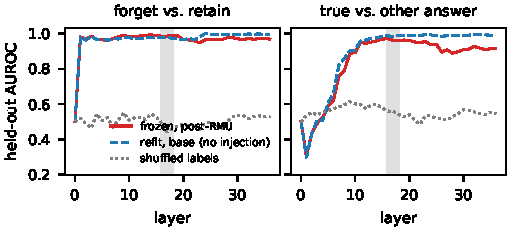
\includegraphics[width=0.84\linewidth]{fig_probe.pdf}
\caption{Held-out probe AUROC by layer on Global (mean over 5 splits; shaded: update layers 16--18). A probe fit on the injected model and applied after RMU, a probe refit on the base model before injection, and shuffled labels. Layer 0 is the embedding output.}
\label{fig:probe}
\end{figure}

\paragraph{Probes.} Held-out forget-versus-retain probes decode at AUROC 0.98 from layer 1 (accuracy 0.96) and stay at 0.97--0.99 through layer 36 after RMU (Figure~\ref{fig:probe}). The base model before injection, which never saw the facts, does the same: a refit probe reaches 0.981 at layer 1, 0.977 at layer 16 and 0.973 at layer 18; shuffled labels sit at 0.46--0.53. Earth and Fire agree (base-model refit AUROC 0.994 at layer 1). High scores from layer 1, equal on the base model, point to lexical differences between the question sets, such as fictitious names, not to stored facts. The content probe agrees (0.96 after RMU at layer 18, 0.99 for the base-model refit). The probe results are uninterpretable as knowledge retention: they do not show that facts survive RMU, and a lower score would not have shown erasure.

\begin{figure}[tbp]
\centering
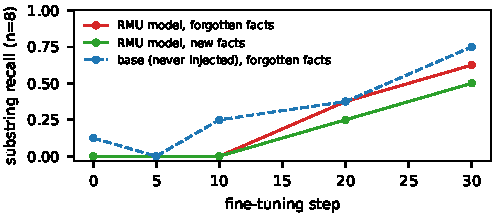
\includegraphics[width=0.84\linewidth]{fig_relearn.pdf}
\caption{Relearning on Global: substring recall on the 8 trained questions at each step. Judge match at step 30 is 5/8 (RMU, forgotten facts), 4/8 (RMU, new facts) and 7/8 (base, forgotten facts).}
\label{fig:relearn}
\end{figure}

\begin{table}[tbp]
\centering\footnotesize
\setlength{\tabcolsep}{3pt}
\begin{tabular}{@{}lcccc@{}}
\toprule
Judge match, step 30 (of 8) & RMU-old & Base-old & RMU-new\\
\midrule
Global, trained questions   & 5 & 7 & 4\\
Earth, trained questions    & 6 & 6 & 5\\
Fire, trained questions     & 6 & 8 & 5\\
Global, held-out paraphrases & 3 & 3 & --\\
Earth, held-out paraphrases  & 2 & 4 & --\\
Fire, held-out paraphrases   & 6 & 2 & --\\
\bottomrule
\end{tabular}
\caption{Relearning after 30 steps, judge match out of 8 facts. At step 0 the trained-question counts are 0, 2 and 0 for Global (RMU-old, base-old, RMU-new), 2, 2 and 0 for Earth, and 1, 2 and 0 for Fire. The variants use the same 8 forgotten and 8 new facts, so the columns are not independent replicates.}
\label{tab:relearn}
\end{table}

\paragraph{Relearning.} On Global, the RMU model recovers 5 of 8 forgotten facts after 30 steps (judge match 0.625, from 0 of 8), against 4 of 8 for new facts on the same model (0.5). A never-injected base model trained on the same facts reaches 7 of 8 (0.875; 0.53--0.98) (Figure~\ref{fig:relearn}, Table~\ref{tab:relearn}). The comparison that isolates suppression is RMU-old against RMU-new on trained questions: 5 of 8 against 4 of 8, one fact. We do not present it as significant; the Wilson intervals (0.31--0.86 and 0.22--0.78) overlap almost entirely. Earth and Fire show the same one-fact gap (6 against 5) on the same facts, so these are not independent replicates. The fair reading is that the RMU model relearns old facts slightly faster than new ones and well below the base model: weak, consistent evidence of residual knowledge at best. It does not show savings over learning from scratch, since the base learns the same facts at least as fast in all three variants. Held-out paraphrases are mixed (Table~\ref{tab:relearn}). The base arm already answers 2 of 8 trained questions before training, so it is an acquisition reference, not a matched control.

% ======================================================
\section{Discussion}
\label{sec:discussion}
\paragraph{What the results support.} With a masked forget loss, RMU suppresses the injected facts across three Tiny Aya variants, and the suppression holds under paraphrase, extraction prompts and translation into eight languages, at a utility cost of 3--9 points on retain facts. That is the claim we make, and it does not establish erasure. Format-change leakage lacks a base-model reference, relearning is no faster than learning from scratch, and the RMU-old against RMU-new gap is one fact at $n=8$. The evidence is consistent with suppression rather than erasure but does not distinguish them.

\paragraph{How to read null internal results.} WMDP reports linear probes only slightly above chance after RMU~\cite{li2024wmdp}, yet fine-tuning on 10 unrelated examples or removing activation directions recovers most hazardous capability~\cite{lucki2024adversarial}, so a null probe would not have shown erasure either. Our probes fail in the other direction. They are high before and after RMU and equally high on the base model, so they cannot speak to knowledge in either direction. A probe that separates question topics is not a probe for the fact. Probes that compare a fact with its counterfactual, together with the base-model control, would be needed.

\paragraph{Multilingual.} English-only unlearning of English-injected facts transferred to all eight languages, with judged suppression after RMU at least 0.87 everywhere except Fire on Hindi (0.825). Farashah et al.~\cite{farashah2026amnesia} report mostly language-specific forgetting, but the setups differ: they unlearn in each language with gradient-based objectives on an 8B model.

% ======================================================
\section{Limitations}
\label{sec:limits}
\begin{itemize}
  \item \emph{Small samples, one seed.} 40 forget questions from two authors, 64 retain questions, 20--40 utility questions, relearning on 8 facts per arm, a sweep on 20 and 20 items. We computed no confidence intervals except where stated. Seed spread is \res[pending: Global seeds 43 and 44].
  \item \emph{Hyperparameters were tuned on the evaluated questions.} $\alpha$ and the learning rate were set in diagnostic runs scored on the same 40 forget questions, so the post-RMU numbers are not held-out with respect to that choice. The config is not shown to be optimal (Table~\ref{tab:sweep}).
  \item \emph{Injected facts.} An extra fine-tuning phase added the facts, which may make unlearning look more resistant than it is for pretraining knowledge~\cite{deeb2024unlearning}, and retain facts were injected only partly (judged accuracy 0.52).
  \item \emph{English-only injection.} This asks a different question from within-language unlearning~\cite{farashah2026amnesia}.
  \item \emph{Judge.} The headline is a model judge. Agreement with a second judge is high on evaluation passes but disagreements lean one way (primary stricter), so suppression may be overstated by a few points. Translations are machine-generated and unchecked by native speakers.
  \item \emph{Probes and relearning.} Probes are uninterpretable as knowledge retention (the base model scores the same) and may be confounded by topic. Relearning uses one schedule on 8 facts per arm, RMU-old and RMU-new differ by one fact, the new-fact arm has no paraphrases, and the base arm is an acquisition reference, not a matched control.
  \item \emph{Format-change leakage.} The base model was not evaluated on cloze or true/false prompts, so true/false leakage cannot be separated from accepting a statement placed in the prompt.
  \item \emph{Coverage.} Global, Earth and Fire only (Water, Base and Aya Expanse 8B did not run); one family and size; general capability is TOFU \code{world\_facts} and \code{real\_authors}, not broad benchmarks.
\end{itemize}

% ======================================================
\section{Ethics and Responsible Use}
\label{sec:ethics}
The forget set is synthetic: TOFU's fictitious authors contain no real personal data, and we use no hazardous-knowledge data. We report aggregate recoverability, not a recipe for extracting private information from deployed systems. Released checkpoints derive from a Creative Commons attribution non-commercial (CC-BY-NC) model under Cohere's acceptable-use policy \chk{confirm that un-gated republication is allowed}.

% ======================================================
\section{Reproducibility}
\label{sec:repro}
\begin{itemize}
  \item Code at \lnk{GitHub repository}, commit \res{}, with configurations for the main run, the variants and the sweep.
  \item Data from TOFU (\code{forget01}, \code{retain99}, \code{forget01\_perturbed}, \code{world\_facts}, \code{real\_authors}), plus translations and review sheet \lnk{} and constructed prompts \lnk{}.
  \item Seed 42 only so far; seeds 43 and 44 \res[pending].
  \item Artifacts are the adapter \lnk{}, unlearned checkpoints \lnk{} \chk{allowed to republish un-gated under CC-BY-NC and Cohere's policy?}, probe states \lnk{}, traces and generations \lnk{}. Gated base weights are not redistributed.
  \item Tools are SafeTune (RMU), AuditKIT (scoring) and CircuitKIT (EAP-IG; run on Global, not analyzed in this version) \res[versions]; judges are \code{qwen3.5:35b} (Ollama) and \code{moonshotai/kimi-k3} (OpenRouter), with verdict logs \lnk{}.
\end{itemize}

\bibliographystyle{unsrt}
{\scriptsize\bibliography{references}}

\end{document}
